\documentclass{standalone}
\usepackage{pgfplots}
\usepackage{sansmath}
\pgfplotsset{compat=1.16}
\definecolor{itoa}{HTML}{3366FF}
\definecolor{std}{HTML}{949494}
\definecolor{bg}{HTML}{CFCFCF}
\begin{document}
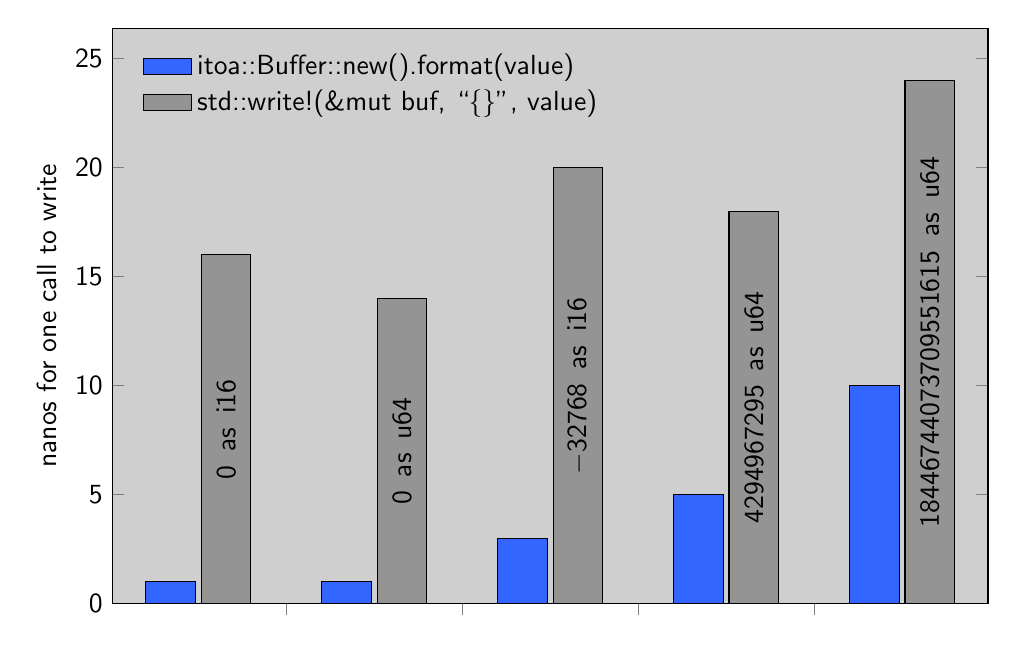
\begin{tikzpicture}
\edef\entries{
  "$0${\enspace}as{\enspace}i16",
  "$0${\enspace}as{\enspace}u64",
  "$-32768${\enspace}as{\enspace}i16",
  "$4294967295${\enspace}as{\enspace}u64",
  "$18446744073709551615${\enspace}as{\enspace}u64",
}
\begin{axis}[
  width=5in,
  height=3.5in,
  ybar,
  ymin=0,
  bar width=18pt,
  enlarge x limits={abs=31pt},
  ylabel={nanos for one call to write},
  legend style={
    anchor=north west,
    at={(0.025,0.975)},
    legend columns=1,
    draw=none,
    fill=none,
  },
  legend entries={
    itoa::Buffer::new().format(value)\\
    std::write!(\&mut buf, ``\{\}'', value)\\
  },
  legend cell align=left,
  xtick={-0.5,0.5,1.5,2.5,3.5,4.5},
  xticklabels={},
  xtick pos=left,
  visualization depends on={y \as \rawy},
  every node near coord/.append style={
    shift={(axis direction cs:0,-\rawy/2)},
    rotate=90,
    anchor=center,
    font=\sansmath\sffamily,
  },
  axis background/.style={fill=bg},
  tick label style={font=\sansmath\sffamily},
  every axis label={font=\sansmath\sffamily},
  legend style={font=\sansmath\sffamily},
  label style={font=\sansmath\sffamily},
]
  \addplot[
    black,
    fill=itoa,
    area legend,
    nodes near coords={},
  ] coordinates {
    (0, 1)
    (1, 1)
    (2, 3)
    (3, 5)
    (4, 10)
  };
  \addplot[
    black,
    fill=std,
    area legend,
    nodes near coords=\pgfmathsetmacro{\input}{{\entries}[\coordindex]}\input,
  ] coordinates {
    (0, 16)
    (1, 14)
    (2, 20)
    (3, 18)
    (4, 24)
  };
\end{axis}
\end{tikzpicture}
\end{document}
